\iffalse
\def\mytitle{MATRICES USING PYTHON}
\def\myauthor{R.Ramesh}
\def\contact{rameshrandhiglra@gmail.com}
\def\mymodule{Future Wireless Communication (FWC)}
\documentclass[10pt, a4paper]{article}
\usepackage[a4paper,outer=1.5cm,inner=1.5cm,top=1.75cm,bottom=1.5cm]{geometry}
\twocolumn
\usepackage{graphicx}
\graphicspath{{./images/}}
\usepackage[colorlinks,linkcolor={black},citecolor={blue!80!black},urlcolor={blue!80!black}]{hyperref}
\usepackage[parfill]{parskip}
\usepackage{lmodern}
\usepackage{tikz}
	\usepackage{physics}
%\documentclass[tikz, border=2mm]{standalone}
\usepackage{karnaugh-map}
%\documentclass{article}
\providecommand{\sbrak}[1]{\ensuremath{{}\left.#1\right]}}
\usepackage{tabularx}
\usepackage{circuitikz}
\usetikzlibrary{calc}
\usepackage{amssymb,amsfonts,amsthm,amsmath}
\newcommand{\myvec}[1]{\ensuremath{\begin{pmatrix}#1\end{pmatrix}}}
\usepackage{amssymb}
\renewcommand*\familydefault{\sfdefault}
\usepackage{watermark}
\usepackage{lipsum}
\usepackage{xcolor}
\usepackage{listings}
\usepackage{float}
\usepackage{titlesec}
\usepackage{amssymb,amsfonts,amsthm,amsmath}
\usepackage{cite}
\usepackage{amssymb,amsfonts,amsthm,amsmath}
\usepackage{algorithmic}
\usepackage{graphicx}
\usepackage{textcomp}
\usepackage{xcolor}
\usepackage{txfonts}
\usepackage{listings}
\usepackage{enumitem}
\usepackage{mathtools}
\usepackage{gensymb}
\usepackage{bm}
\usepackage{polynom}

\providecommand{\res}[1]{\Res\displaylimits_{#1}} 
%\providecommand{\norm}[1]{\lVert#1\rVert}
\providecommand{\mtx}[1]{\mathbf{#1}}
\providecommand{\fourier}{\overset{\mathcal{F}}{ \rightleftharpoons}}
%\providecommand{\hilbert}{\overset{\mathcal{H}}{ \rightleftharpoons}}
\providecommand{\system}{\overset{\mathcal{H}}{ \longleftrightarrow}}
	%\newcommand{\solution}[2]{\textbf{Solution:}{#1}}
\newcommand{\solution}{\noindent \textbf{Solution: }}
\newcommand{\cosec}{\,\text{cosec}\,}
\newcommand{\mydet}[1]{\ensuremath{\begin{vmatrix}#1\end{vmatrix}}}
	\newcommand*{\permcomb}[4][0mu]{{{}^{#3}\mkern#1#2_{#4}}}
\newcommand*{\perm}[1][-3mu]{\permcomb[#1]{P}}
\newcommand*{\comb}[1][-1mu]{\permcomb[#1]{C}}
\providecommand{\fourier}{\overset{\mathcal{F}}{ \rightleftharpoons}}
%\providecommand{\hilbert}{\overset{\mathcal{H}}{ \rightleftharpoons}}
\providecommand{\system}{\overset{\mathcal{H}}{ \longleftrightarrow}}
\providecommand{\mtx}[1]{\mathbf{#1}}
\titlespacing{\subsection}{1pt}{\parskip}{3pt}
\titlespacing{\subsubsection}{0pt}{\parskip}{-\parskip}
\titlespacing{\paragraph}{0pt}{\parskip}{\parskip}
\newcommand{\figuremacro}[5]{
    \begin{figure}[#1]
        \centering
        \includegraphics[width=#5\columnwidth]{#2}
        \caption[#3]{\textbf{#3}#4}
        \label{fig:#2}
    \end{figure}
}

\let\vec\mathbf
\lstset{
frame=single, 
breaklines=true,
columns=fullflexible
}
%\thiswatermark{\centering \put(0,-90.0){\includegraphics[scale=0.5]{iit h.png}} }
\title{\mytitle}
\author{\myauthor\hspace{1em}\\\contact\\FWC22076\hspace{6.5em}IITH\hspace{0.5em}\mymodule\hspace{6em}September}
\date{}


\begin{document}
\maketitle
\paragraph{\textit{\large Problem statement: }\\
\fi
 By using the concept of equation of a line, prove that the three points (3, 0), (– 2, – 2) and (8, 2) are collinear.
	\begin{figure}[!ht]
		\centering
 \includegraphics[width=\columnwidth]{chapters/11/10/2/20/figs/figs6.pdf}
		\caption{}
		\label{fig:11/10/2/20}
  	\end{figure}
	\\
	\solution 
 \iffalse
 \section*{Construction}
 	\begin{center}
\textsl{}  \includegraphics[scale=0.49]{figs6.pdf}
  
  Figure of construction
  	\end{center}
The input parameters for this construction are 
\begin{center}
\begin{tabular}{|c|c|c|}
	\hline
	\textbf{Symbol}&\textbf{Value}&\textbf{Description}\\
	\hline
	$\vec{A}$&\myvec{3\\0}&collinear point\\[8pt]
	\hline
		$\vec{B}$&\myvec{-2\\-2}&collinear point\\[8pt]
	\hline
		$\vec{C}$&\myvec{8\\2}&collinear point\\[8pt]
	\hline

\end{tabular}
\end{center}
\section*{Solution}
\textbf{Statement:}
the rank of matrix defines number of linearly dependent vectors.  
\\

\begin{align}
	  \vec{D}= \vec{A}- \vec{B}
	  \\
	  = {\myvec{ 3 \\ 0}-\myvec{-2 \\ -2}}
	  \\
	  =\myvec{-5 \\ -2}
 \end{align}
  \begin{align}
	  \vec{E}= \vec{A}- \vec{C}
	  \\
	  ={\myvec{ 8 \\ 2}-\myvec{3 \\ 0}}
	  \\
	  =\myvec{ 5 \\ 2}
  \end{align}
   Now the matrix is:
\begin{equation}
\boldsymbol{F}=
\begin{pmatrix}
 
     \boldsymbol{D} & \boldsymbol{E}
 \end{pmatrix}
 \end{equation}
 \fi
 The collinearity matrix can be expressed as
 \begin{align}
			    \myvec{-5 & -2
			    \\
			    5 & 2 }  
			    \xleftrightarrow[]{R_2 \leftarrow {R_1 + R_2}}
			    \myvec{	    -5 & -2  
			    \\
			    0 & 0}  
\end{align}
which is a rank 1 matrix.
\iffalse
\textbf{}From the above rank of matrix is 1
\\
\textbf{If rank of matrix F is "1"  then the vectors  are in linearly dependent.so points are in collinear.} 
  
\end{document}
\fi
